% 2011 年福建卷理科第 4 题：矩形与三角形 ABE。
% 来源 PDF：普通高考/2011/2011福建理.pdf，SHA-256 1a36c388b64669b29d16fe359efb087d96026059df01d26759f8bb5dd48342f1。
% 原页：第 1 页第 1 栏中部，书页码 659。
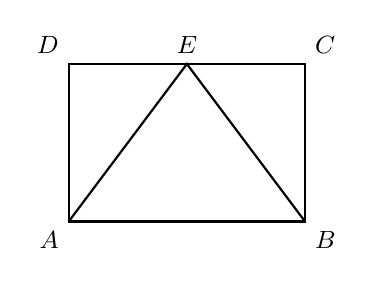
\begin{tikzpicture}[>=stealth, semithick, font=\small, scale=1.0]
  \coordinate (A) at (0,0);
  \coordinate (B) at (3,0);
  \coordinate (C) at (3,2);
  \coordinate (D) at (0,2);
  \coordinate (E) at (1.5,2);
  \draw[thick] (A)--(B)--(C)--(D)--cycle;
  \draw[thick] (A)--(E)--(B);
  \node[below left] at (A) {$A$};
  \node[below right] at (B) {$B$};
  \node[above right] at (C) {$C$};
  \node[above left] at (D) {$D$};
  \node[above] at (E) {$E$};
\end{tikzpicture}
